\documentclass[../../MainTexts/main.tex]{subfiles}


\begin{document}

\section*{Supplementary Figures}
\label{sifigures}


\begin{sifigure}[H]
	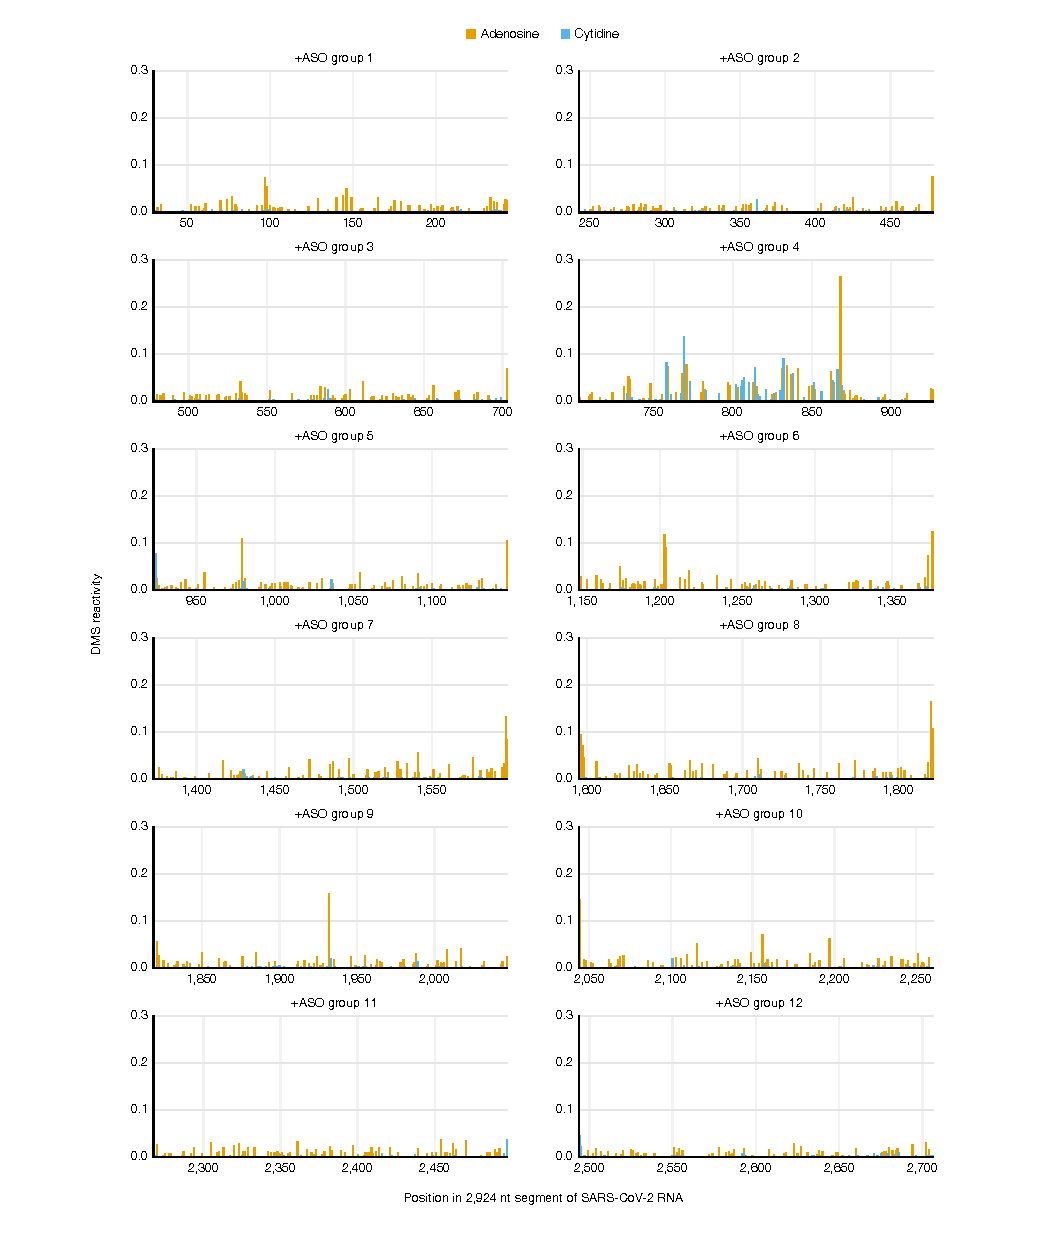
\includegraphics[width=\textwidth]{sars2-tile-target.pdf}
	\caption{\textbf{Mutational profile of each ASO target section upon adding the corresponding group of ASOs to the 2,924 nt segment of SARS-CoV-2 genomic RNA.} Positions are colored based on the RNA sequence.}
	\label{sars2-tile-target}
\end{sifigure}


\begin{sifigure}[H]
	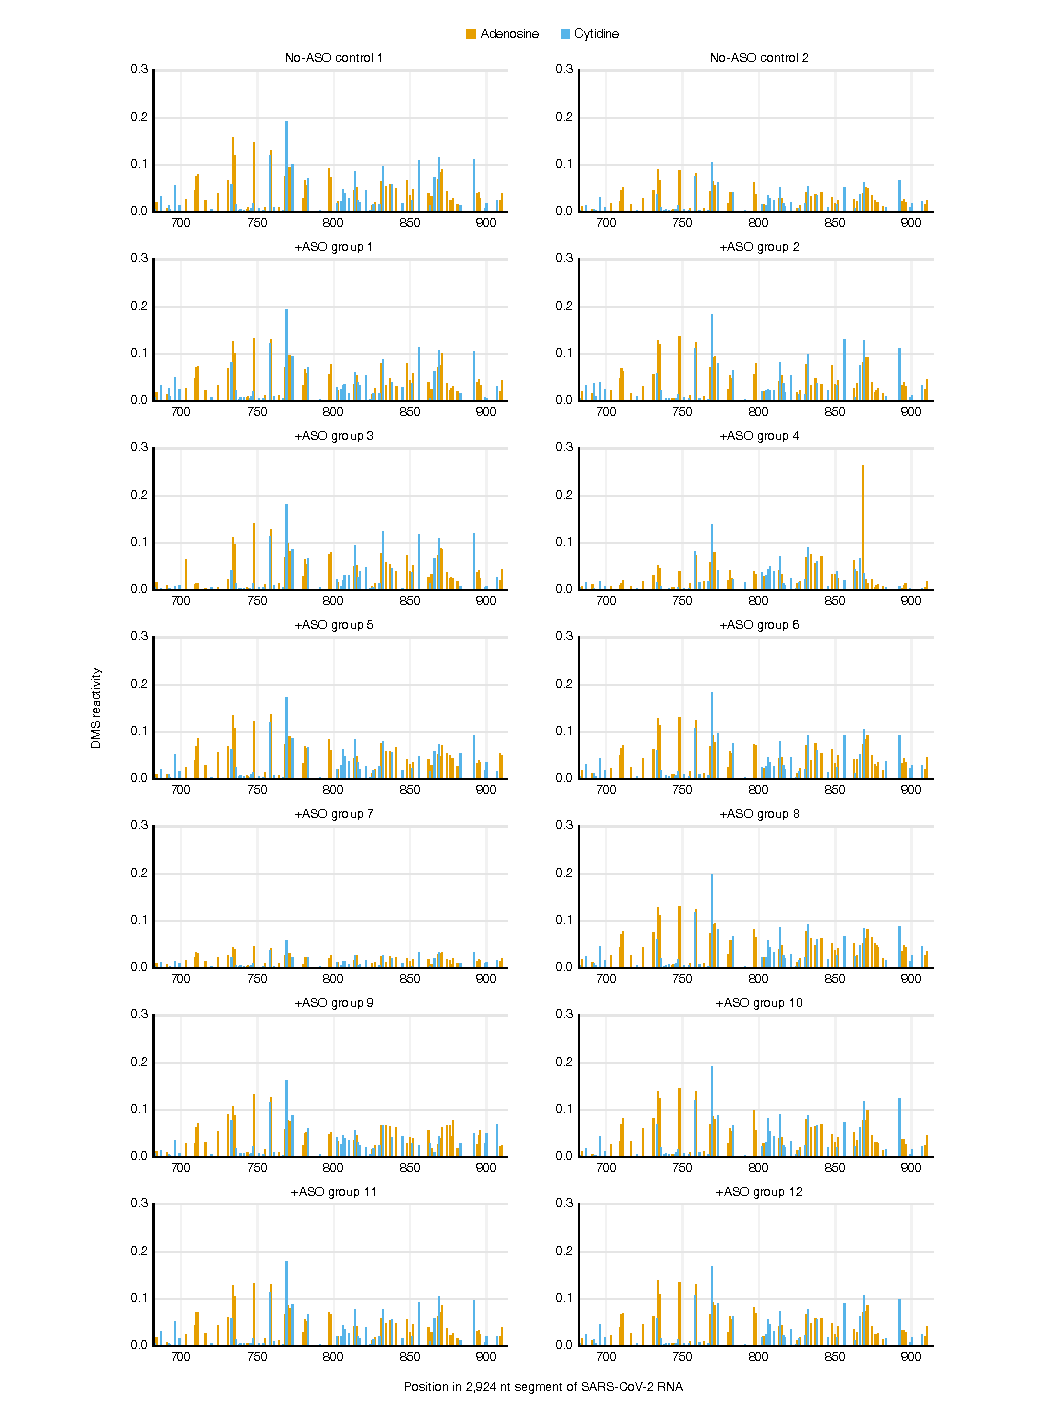
\includegraphics[width=\textwidth]{sars2-tile-fse.pdf}
	\caption{\textbf{Mutational profiles of the FSE section upon adding each group of ASOs to the 2,924 nt segment of SARS-CoV-2 genomic RNA.} Positions are colored based on the RNA sequence.}
	\label{sars2-tile-fse}
\end{sifigure}


\begin{sifigure}[H]
	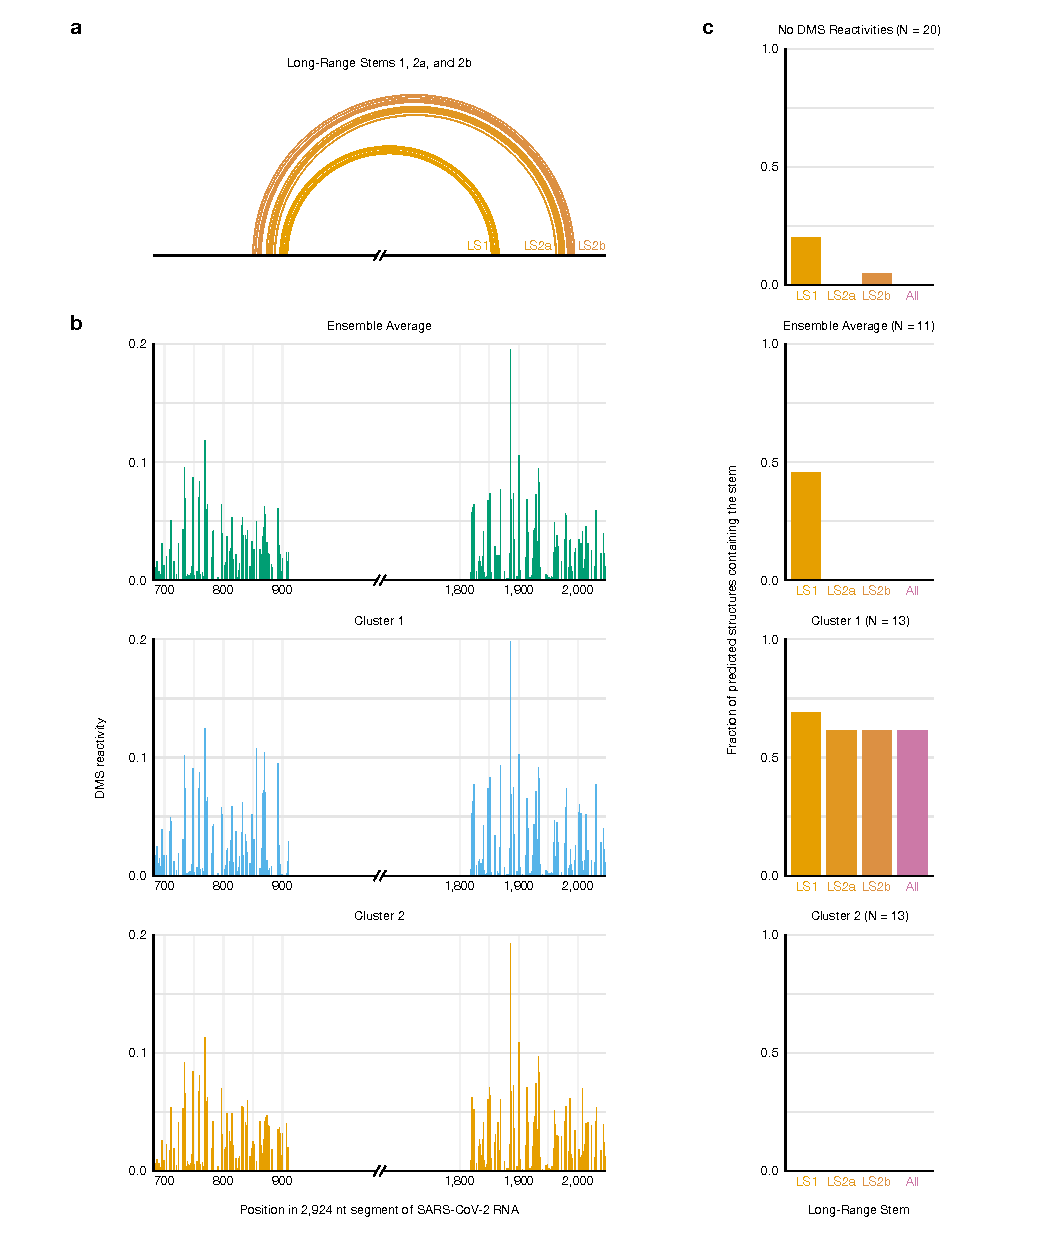
\includegraphics[width=\textwidth]{sars2-clusters-fold.pdf}
	\caption{\textbf{Improved prediction of long-range stems in SARS-CoV-2 using clustered DMS reactivities.} \textbf{(a)}~Model of the two inner stems of the FSE-arch~\cite{Ziv2020}, denoted long stems (LS) 1 and 2a/b. \textbf{(b)}~Mutational profiles of the ensemble average and of clusters 1 and 2 on both sides of the FSE-arch. \textbf{(c)}~For each mutational profile (as well as a purely thermodynamic prediction with no DMS reactivities), the fraction of predicted structures in which each long stem was predicted perfectly (i.e. all base pairs were present). The numbers of predicted structures (N) are indicated.}
	\label{sars2-clusters-fold}
\end{sifigure}


\begin{sifigure}[H]
	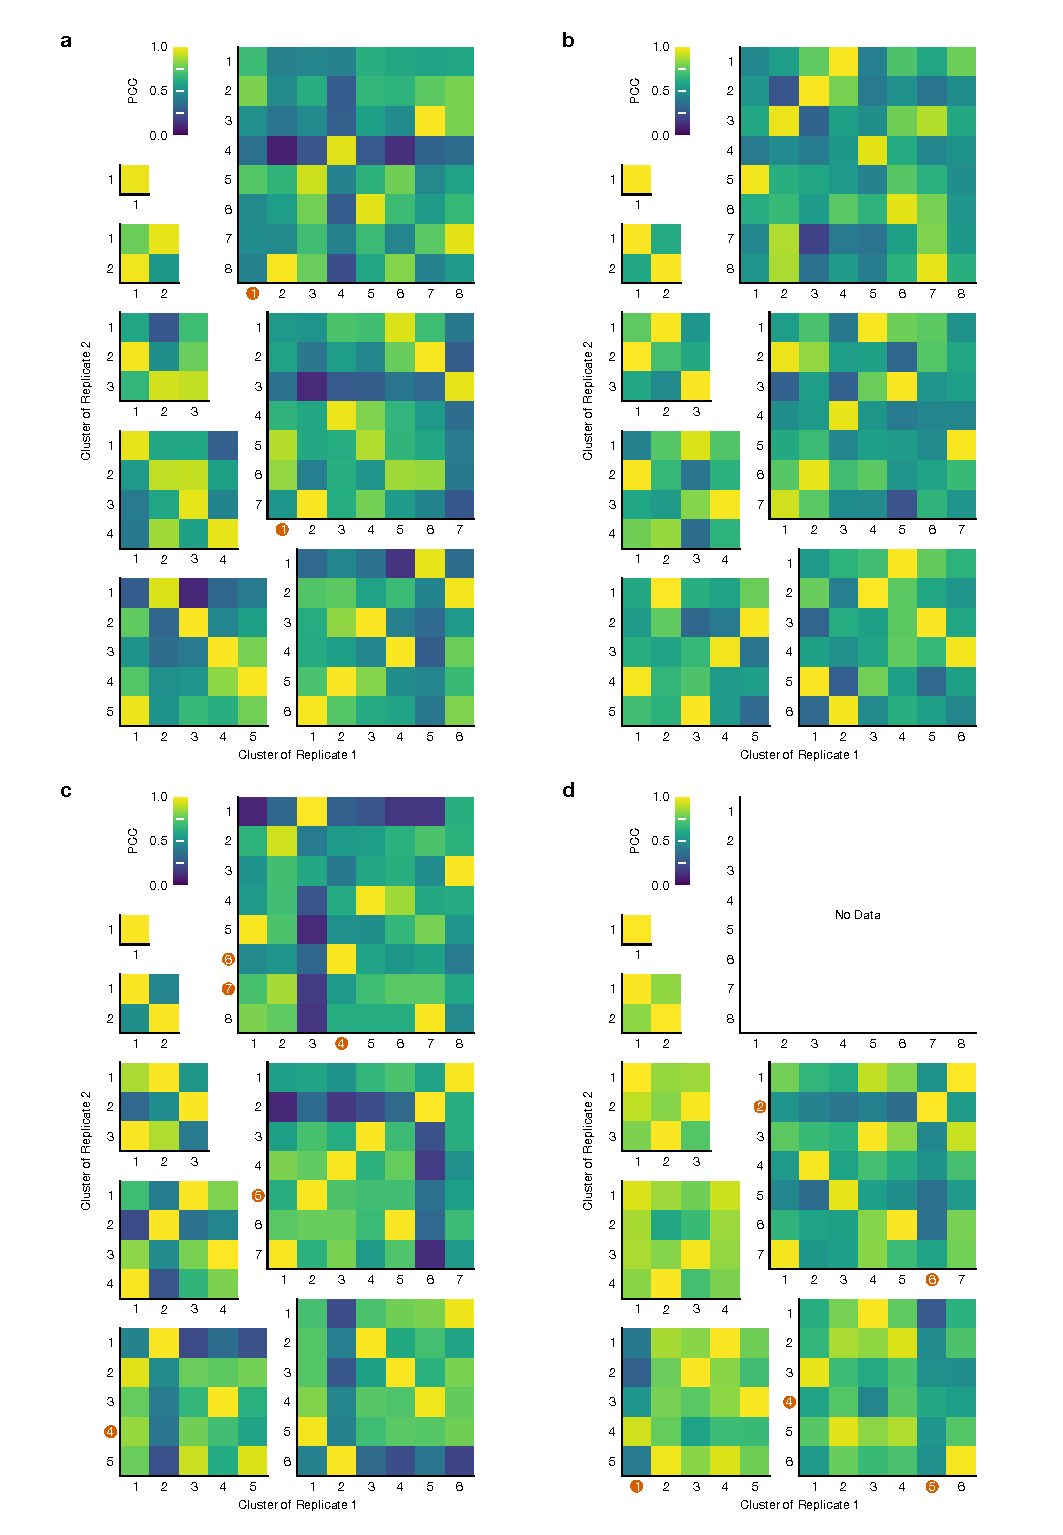
\includegraphics[width=\textwidth]{sars2-compare-clusters.pdf}
	\caption{\textbf{Reproducibility of clustering the SARS-CoV-2 FSE after adding ASOs.} \textbf{(a)}~Heatmaps of the Pearson correlation coefficient (PCC) between each pair of clusters from two replicates of the 1,799 nt segment of SARS-CoV-2. Each heatmap corresponds to one order (i.e. number of clusters). Clusters are marked with red circles if at least one DMS reactivity exceeded 0.3. \textbf{(b)}~Same as (a) plus Anti-AS1 ASO. \textbf{(c)}~Same as (a) plus Anti-PS2-overlap ASO. \textbf{(d)}~Same as (a) plus Anti-AS1 and Anti-PS2-overlap ASOs.}
	\label{sars2-compare-clusters}
\end{sifigure}


\begin{sifigure}[H]
	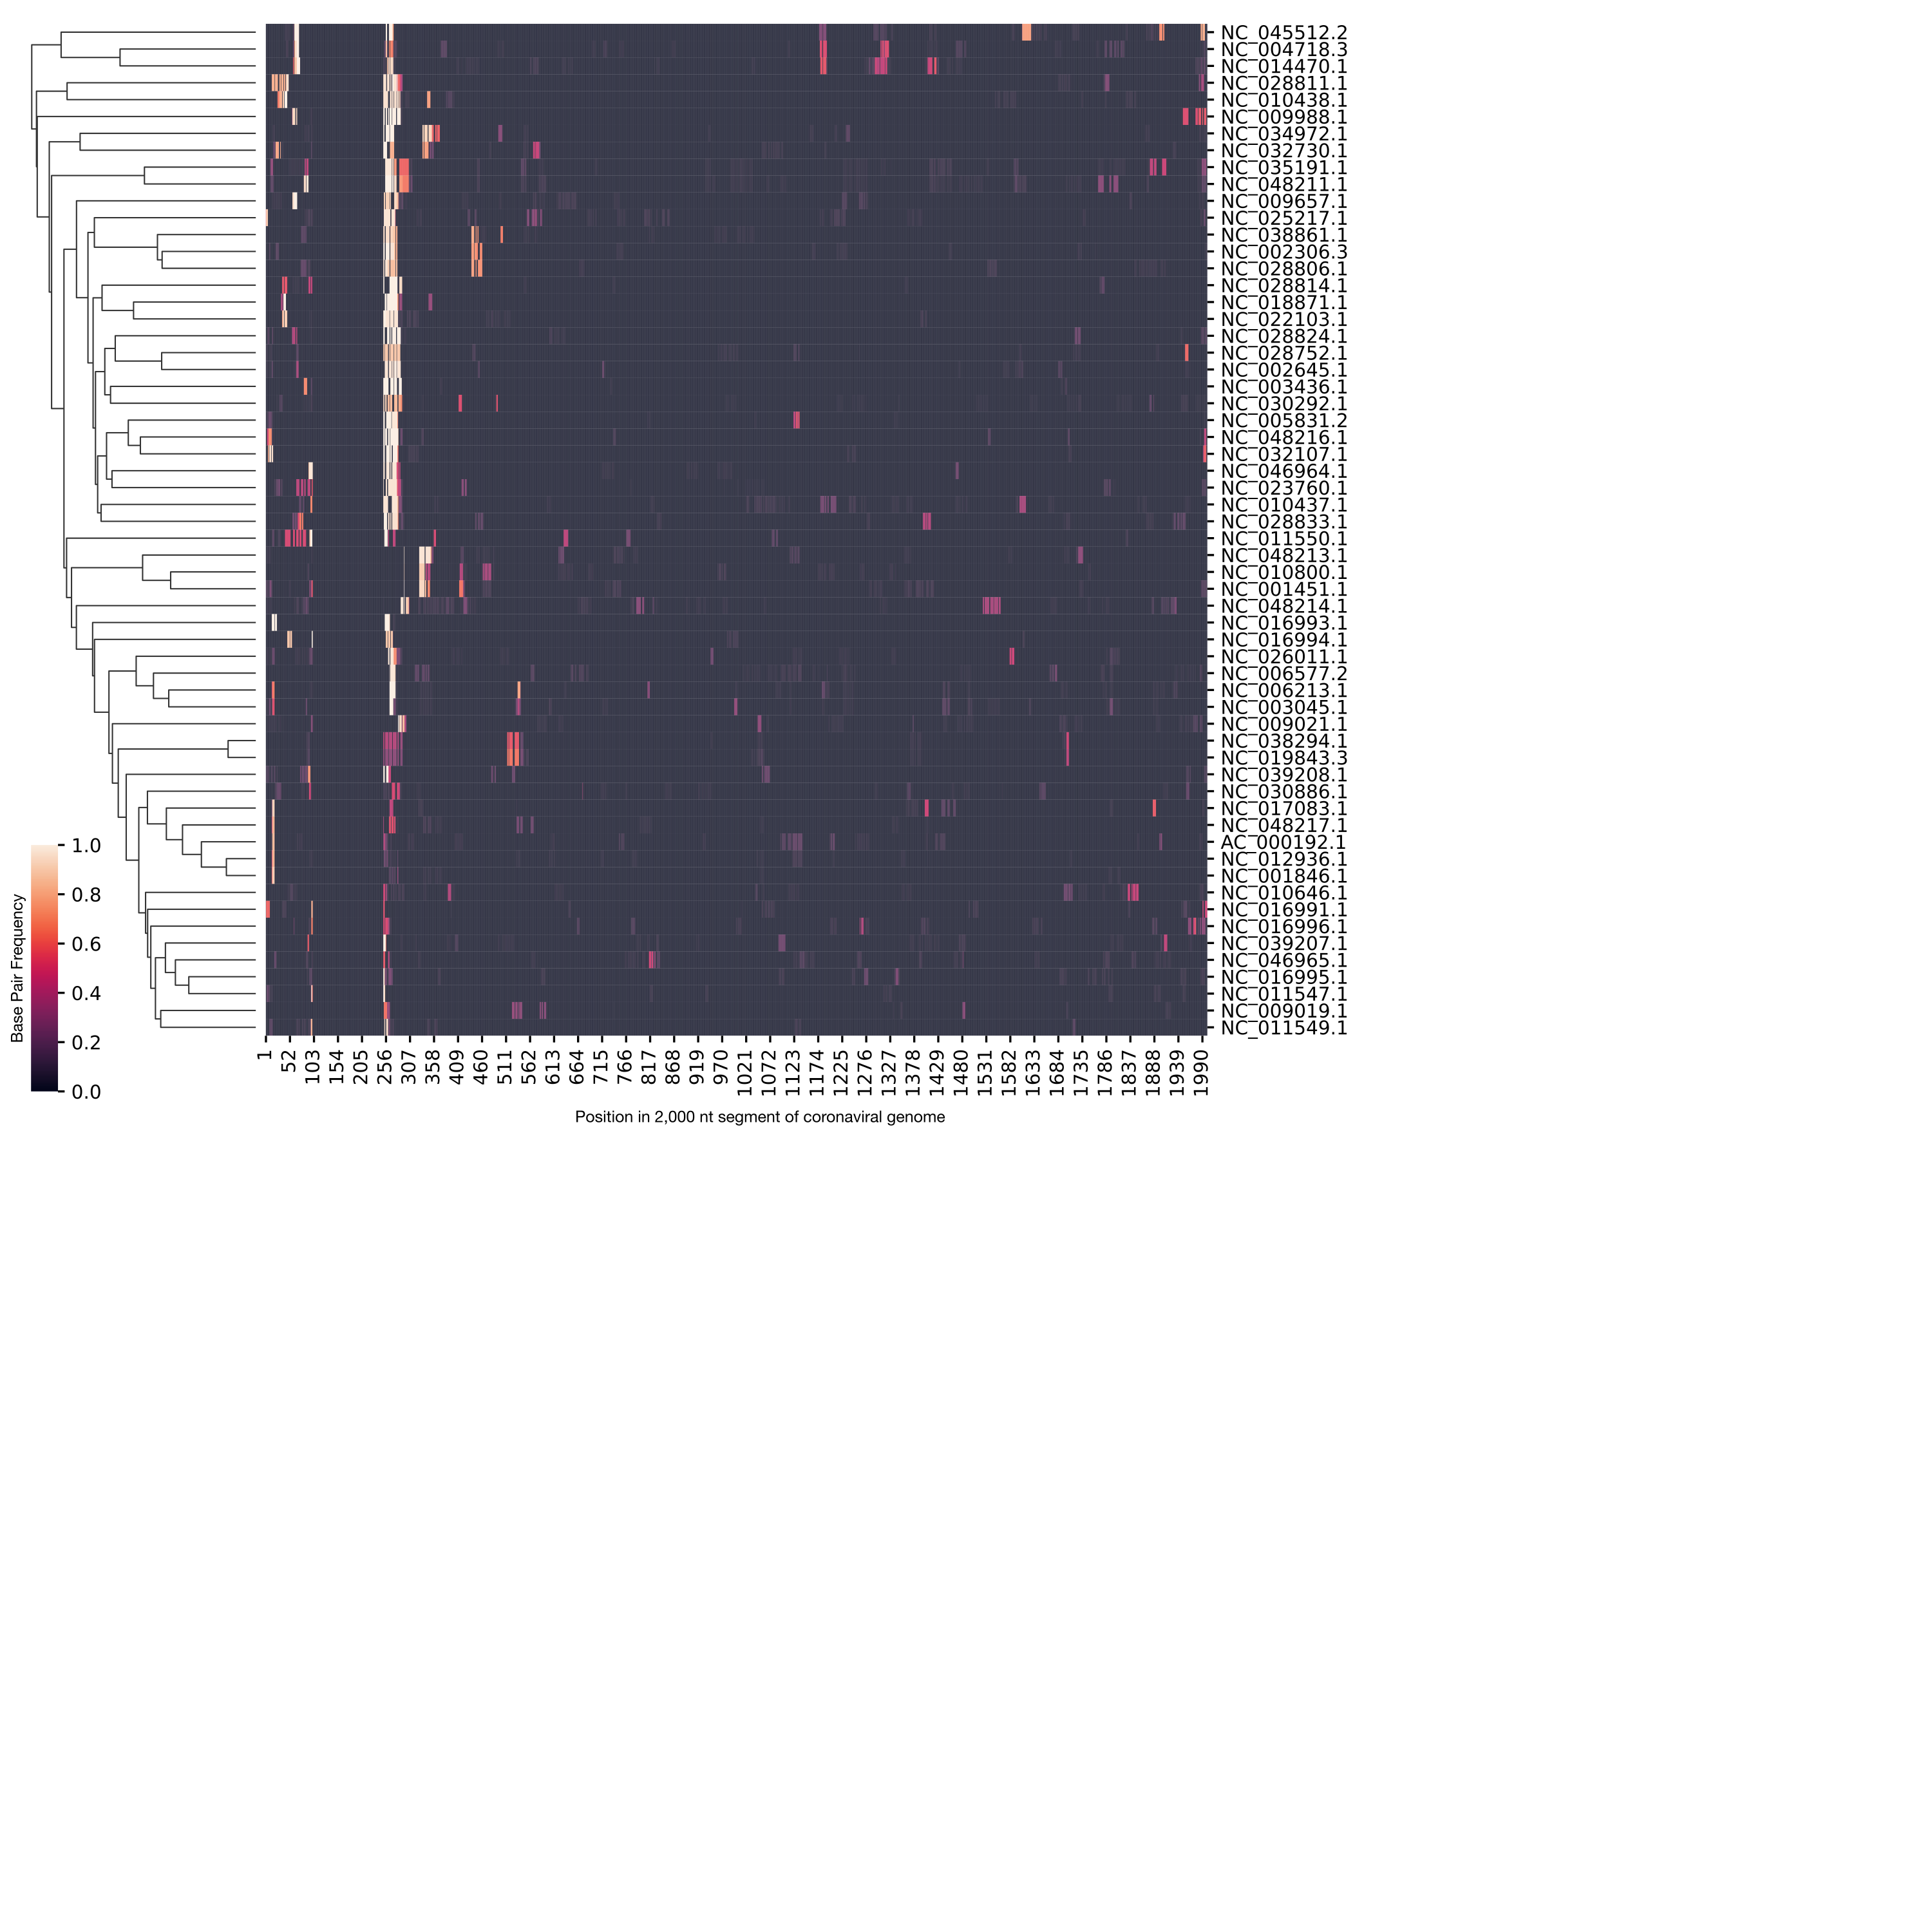
\includegraphics[width=\textwidth]{contact_freqs.png}
	\caption{\textbf{Computational screen of long-range base pairing near the FSE in 60 coronaviruses.} For each 2,000 nt segment of each coronaviral genome, the fraction of predicted structures in which each position outside the range 101-250 base-paired with any position in the range 101-250 is indicated. Genomes are clustered by their base-pairing frequencies. For each genome, the accession number for NCBI~\cite{OLeary2016} is indicated.}
	\label{contact_freqs}
\end{sifigure}


\begin{sifigure}[H]
	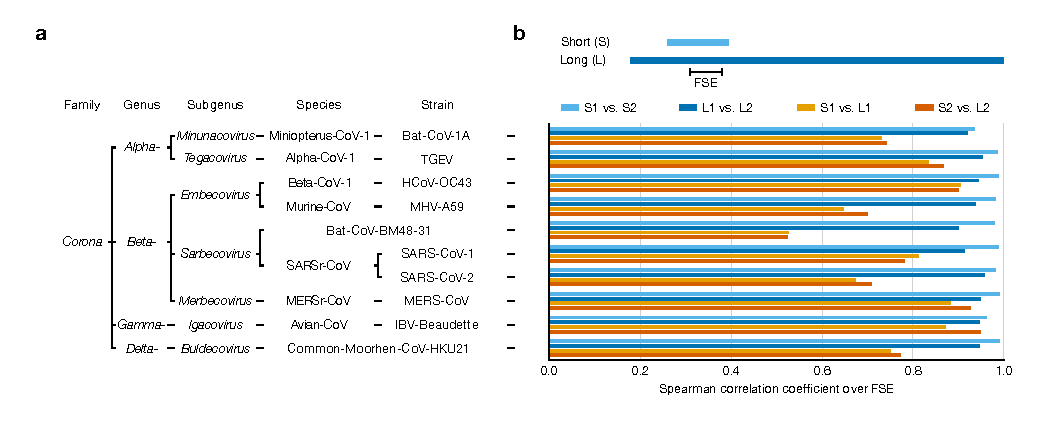
\includegraphics[width=\textwidth]{ten-covs.pdf}
	\caption{\textbf{Experimental screen of long-range base pairing near the FSE in 10 coronaviruses.} \textbf{(a)}~Taxonomy of the ten coronavirus species/strains in this screen; the lowest-level group for each virus is bolded. Bat-CoV-1A: bat coronavirus 1A (NC\_010437.1), TGEV: transmissible gastroenteritis virus (NC\_038861.1), HCoV-OC43: human coronavirus OC43 (NC\_006213.1), MHV-A59: murine hepatitis virus strain A59 (NC\_048217.1), Bat-CoV-BM48-31: bat coronavirus BM48-31 (NC\_014470.1), SARS-CoV-1: severe acute respiratory syndrome coronavirus 1 (NC\_004718.3), SARS-CoV-2: severe acute respiratory syndrome coronavirus 2 (NC\_045512.2), MERS-CoV: Middle East respiratory syndrome coronavirus (NC\_019843.3), IBV-Beaudette: avian infectious bronchitis virus strain Beaudette (NC\_001451.1), Common-Moorhen-CoV-HKU21: common moorhen coronavirus HKU21 (NC\_016996.1). \textbf{(b)}~Spearman correlation coefficients of DMS reactivities over the FSE between replicates 1 and 2 of short (239 nt) and long (1,799 nt) segments of each coronaviral genome.}
	\label{ten-covs}
\end{sifigure}


\begin{sifigure}[H]
	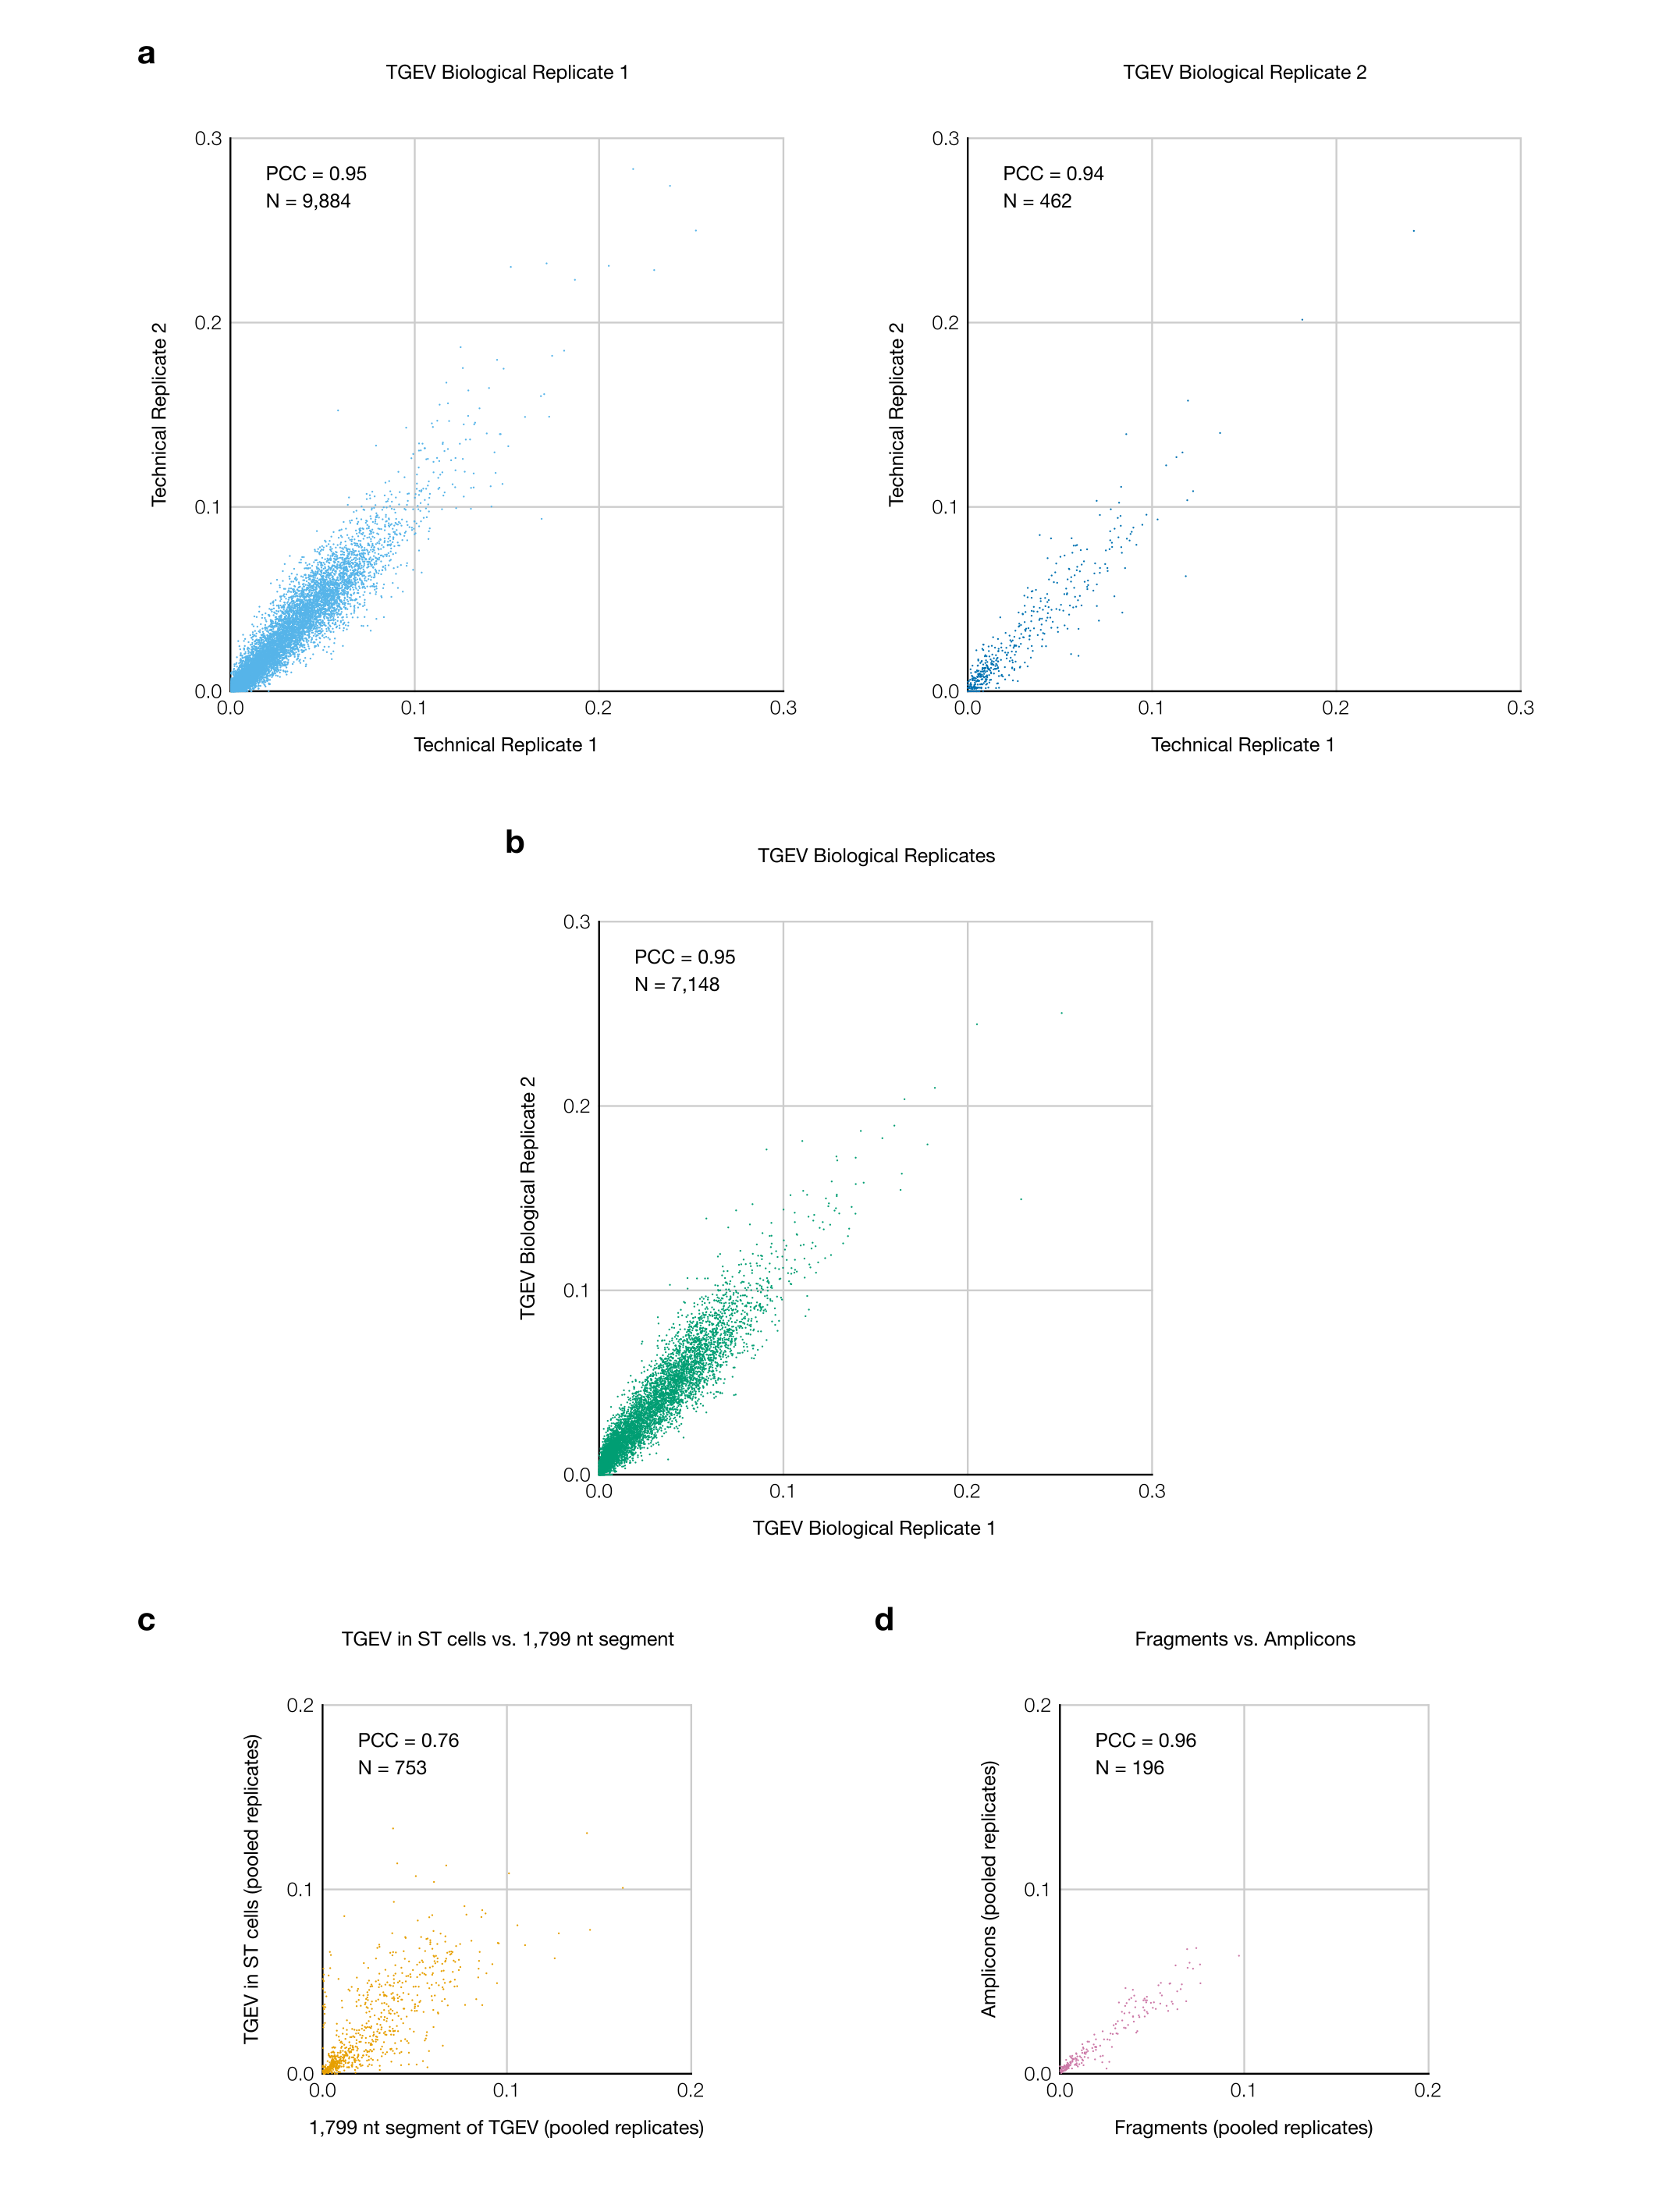
\includegraphics[width=\textwidth]{tgev_reps.pdf}
	\caption{\textbf{Replicates of TGEV in ST cells and comparison to the 1,799 nt segment.} \textbf{(a)}~Comparison of DMS reactivities of the two technical replicates for each biological replicate of TGEV in ST cells. Each point represents one base in the sequence. The number of points (N) and Pearson correlation coefficient (PCC) are indicated for each plot. One point with DMS reactivity exceeding 0.3 in both technical replicates of biological replicate 1 is not shown. \textbf{(b)}~Comparison of DMS reactivities of the two biological replicates (pooled technical replicates). \textbf{(c)}~DMS reactivities of TGEV in ST cells using random fragmentation versus amplicons (pooled biological replicates). \textbf{(d)}~DMS reactivities of TGEV in ST cells (pooled biological replicates) versus the 1,799 nt segment.}
	\label{tgev_reps}
\end{sifigure}


\begin{sifigure}[H]
	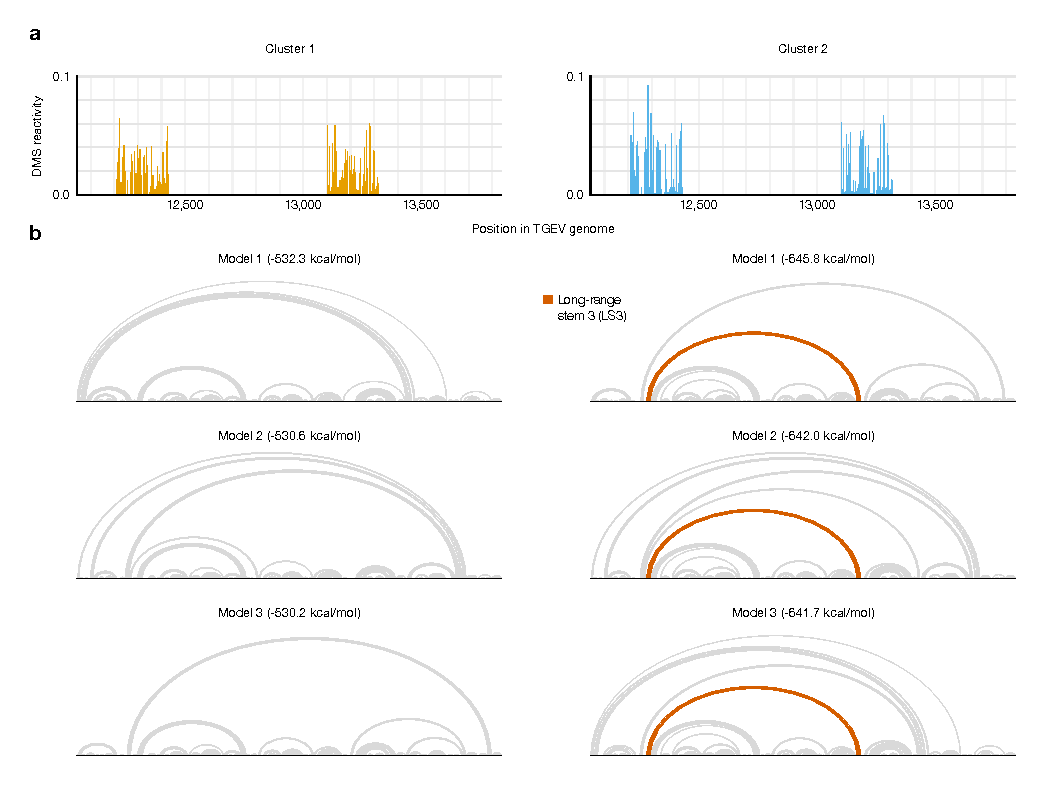
\includegraphics[width=\textwidth]{tgev-clusters.pdf}
	\caption{\textbf{Alternative structures on both sides of the long-range base pairs in TGEV.} \textbf{(a)}~Scatter plots of DMS reactivities over the 3' side of the predicted long-range stem in TGEV (Figure~\ref{covs}) comparing each cluster from amplicons in ST cells to the 1,799~nt segment with ASOs targeting the 5' side of the long-range stem, with Pearson correlation coefficient (PCC) indicated; each point is one base. \textbf{(b)}~Receiver operating characteristic (ROC) curves comparing each cluster from amplicons in ST cells to the structure model of the 1,799~nt segment of TGEV including the long-range base pairs (Figure~\ref{covs}), with area under the curve (AUC) indicated. \textbf{(c)}~DMS reactivities of clusters~1 and~2 and the three lowest-energy structure models of the 1,799~nt segment (positions 12,042-13,840) based on each cluster. Long-range stem~3 (LS3) is highlighted when it appears in a model. Structures were drawn with VARNA~\cite{Darty2009}.}
	\label{tgev-clusters}
\end{sifigure}


\begin{sifigure}[H]
	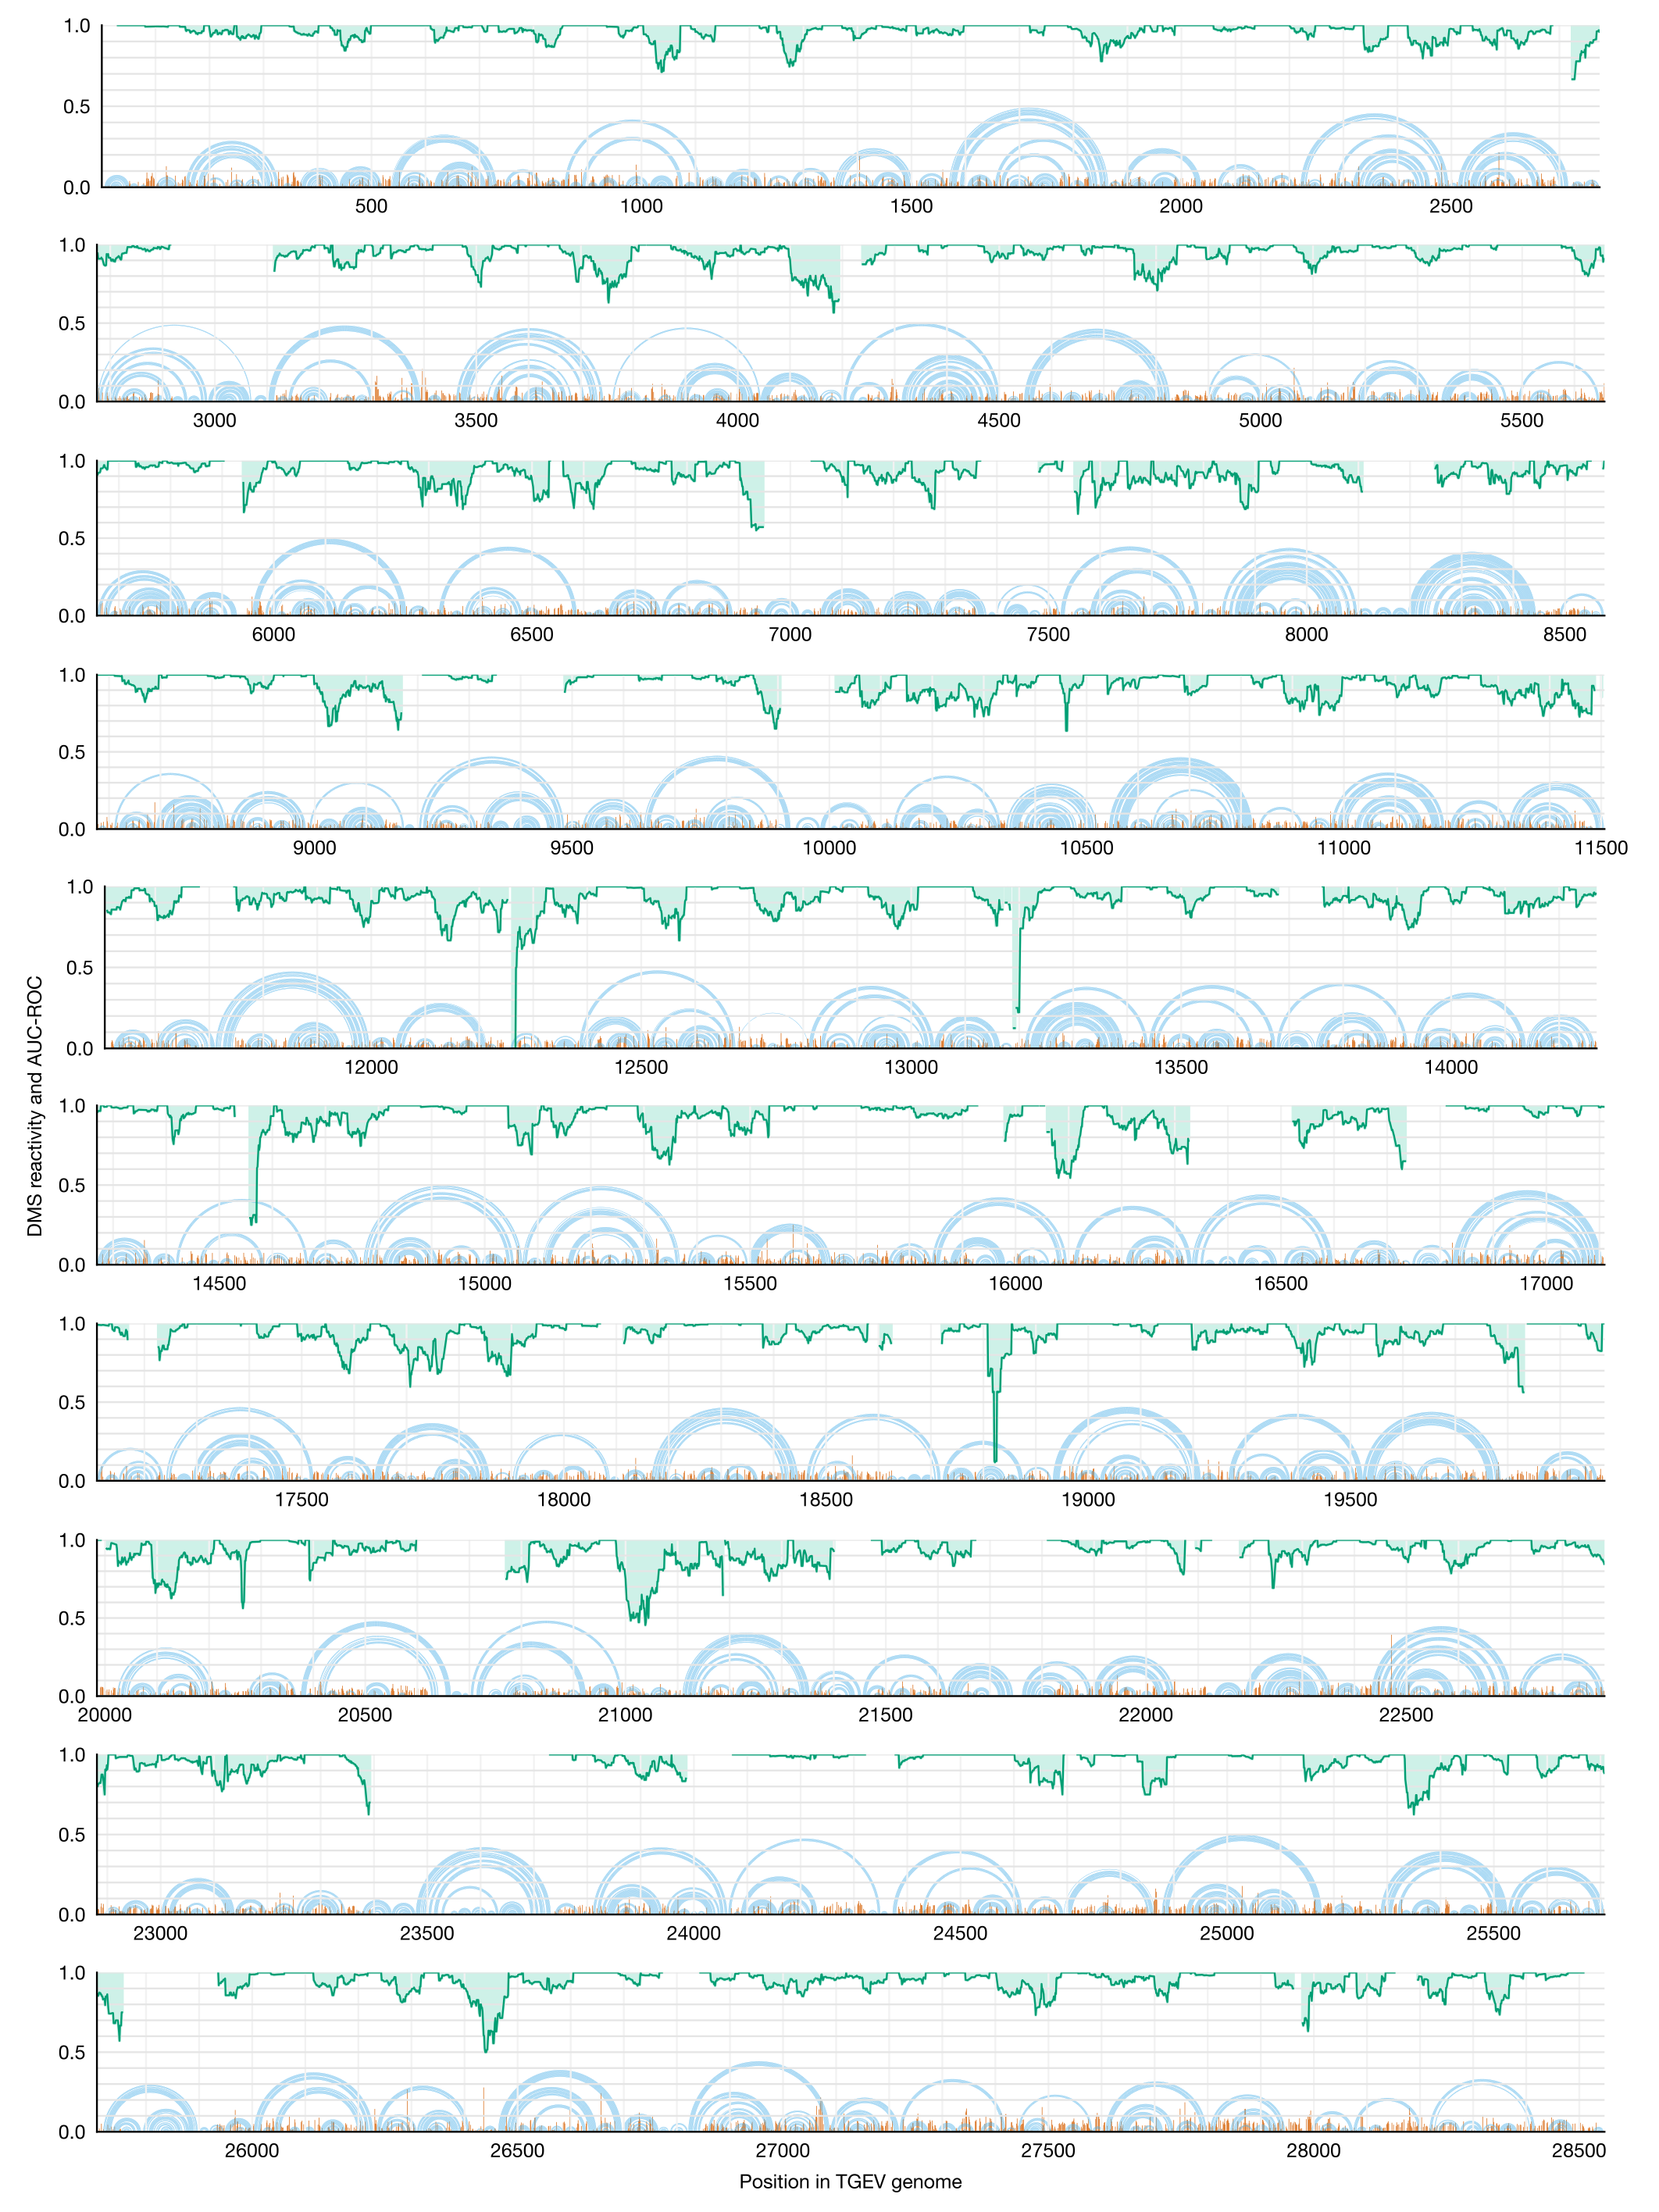
\includegraphics[width=\textwidth]{tgev-full.pdf}
	\caption{\textbf{Short-range base pairs across the full TGEV genome.} Model of the secondary structure of the entire TGEV genome with a maximum distance of 300~nt between paired bases (blue). DMS reactivities used to generate the model are shown in red. Rolling (45~nt) area under the receiver operating characteristic curve (AUC-ROC), measuring how well the secondary structure model fits the DMS reactivities, is shown in green.}
	\label{tgev-full}
\end{sifigure}


\begin{sifigure}[H]
	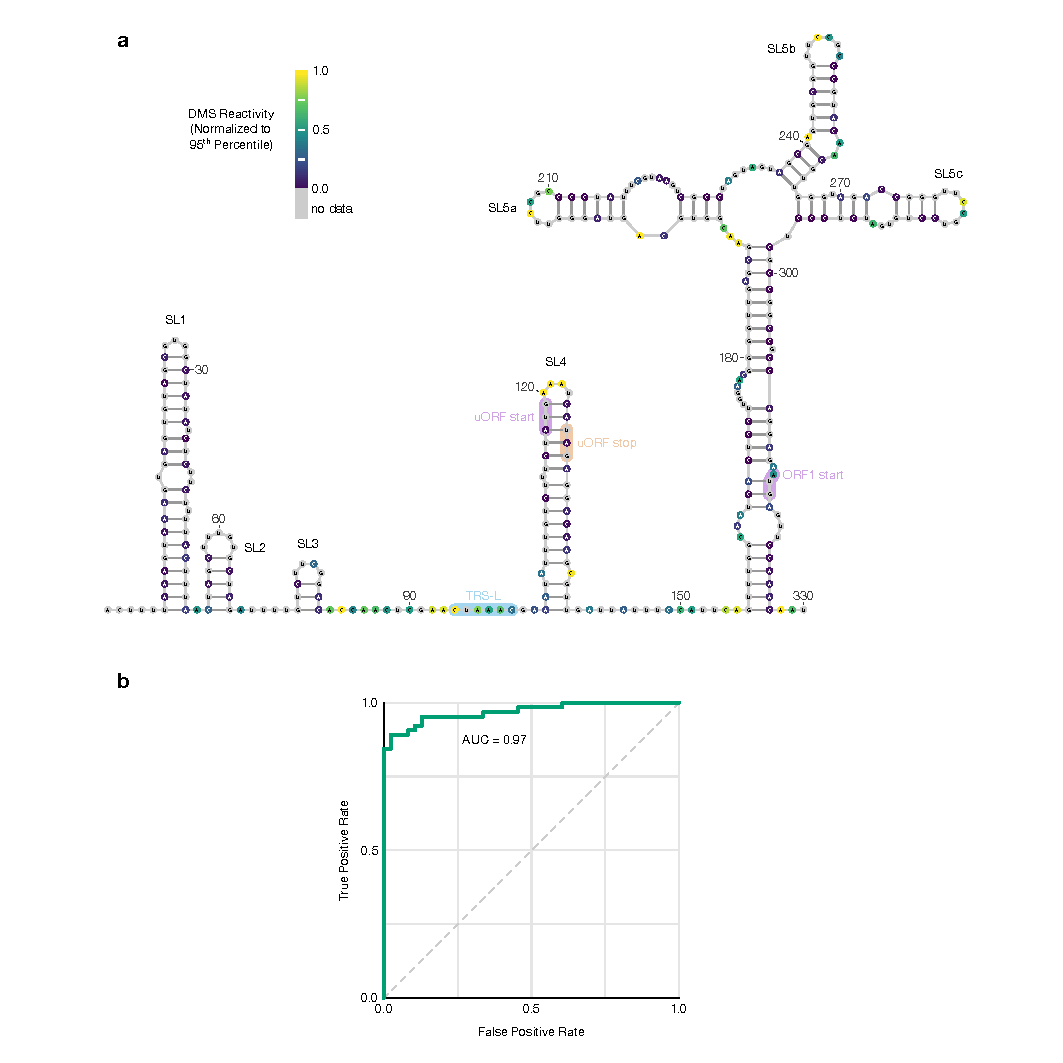
\includegraphics[width=\textwidth]{tgev_5utr.pdf}
	\caption{\textbf{Secondary structure of the TGEV 5' UTR.} \textbf{(a)}~Model of the secondary structure of the first 330 nt of the TGEV genome, based on DMS reactivities in infected ST cells normalized to the 95\textsuperscript{th} percentile. Bases are colored by DMS reactivity. The model includes the conserved stem loops SL1, SL2, SL3, SL4, SL5a, SL5b, and SL5c~\cite{Yang2015a}. The leader transcription regulatory sequence (TRS-L)~\cite{Alonso2002}, upstream open reading frame (uORF)~\cite{Nakagawa2016}, and start codon of ORF1 are also labeled. The model was drawn using VARNA~\cite{Darty2009}. \textbf{(b)}~Receiver operating characteristic curve showing agreement between the DMS reactivities and the secondary structure model; the area under the curve (AUC) is indicated.}
	\label{tgev_5utr}
\end{sifigure}


\end{document}
